% convection, v1.0

\chapter{Convection and the Radon Veto}~\label{ch:convection}

\paragraph{Abstract} While liquid xenon detectors are a mature technology, convection in these devices has not been studied in any depth. In this chapter we provide some background information about convection in liquid xenon as well as the first measurement in XENON1T. We find a single convection cell, as seen in other similar experiments. Additionally, we introduce the ``radon veto'', an analysis that attempts to use knowledge of convection to follow atoms of the uranium decay chain throughout the XENON1T detector and remove the corresponding \Pb~events from the dark matter signal region of interest. This has the potential to significantly boost the sensitivity of the experiment by reducing the background rate of electronic recoils at a marginal cost of exposure.

\section{Introduction}

The analysis of the ${}^{220}$Rn calibration data from XENON100~\cite{Aprile:2016pmc} revealed a buoyancy-driven convection pattern with a considerable $8\1{mm/s}$ fluid speed. A similar analysis from LUX~\cite{Malling:2014} of \Rn~in background data in revealed a pattern with the same features but a higher fluid speed of $3\1{cm/s}$. This was in stark contrast to the lack of convection that was observed in EXO-200~\cite{Albert:2015vma}.

Let us begin with a brief review of the relevant portion of the decay chain of primordial uranium, as shown in Figure~\ref{fig:useries}. \Rn, a noble element, readily diffuses out of the materials, mixes easily with the xenon, and also bypasses the majority of purification systems. \Pb~decays to the ground state of $^{214}$Bi with a branching ratio of $11.0\%$, and a fraction of these decays lie in the dark matter signal region of interest. These events are the primary source of background in this energy range~\cite{Aprile:2015uzo}.

\begin{figure}[htb]
    \centering
    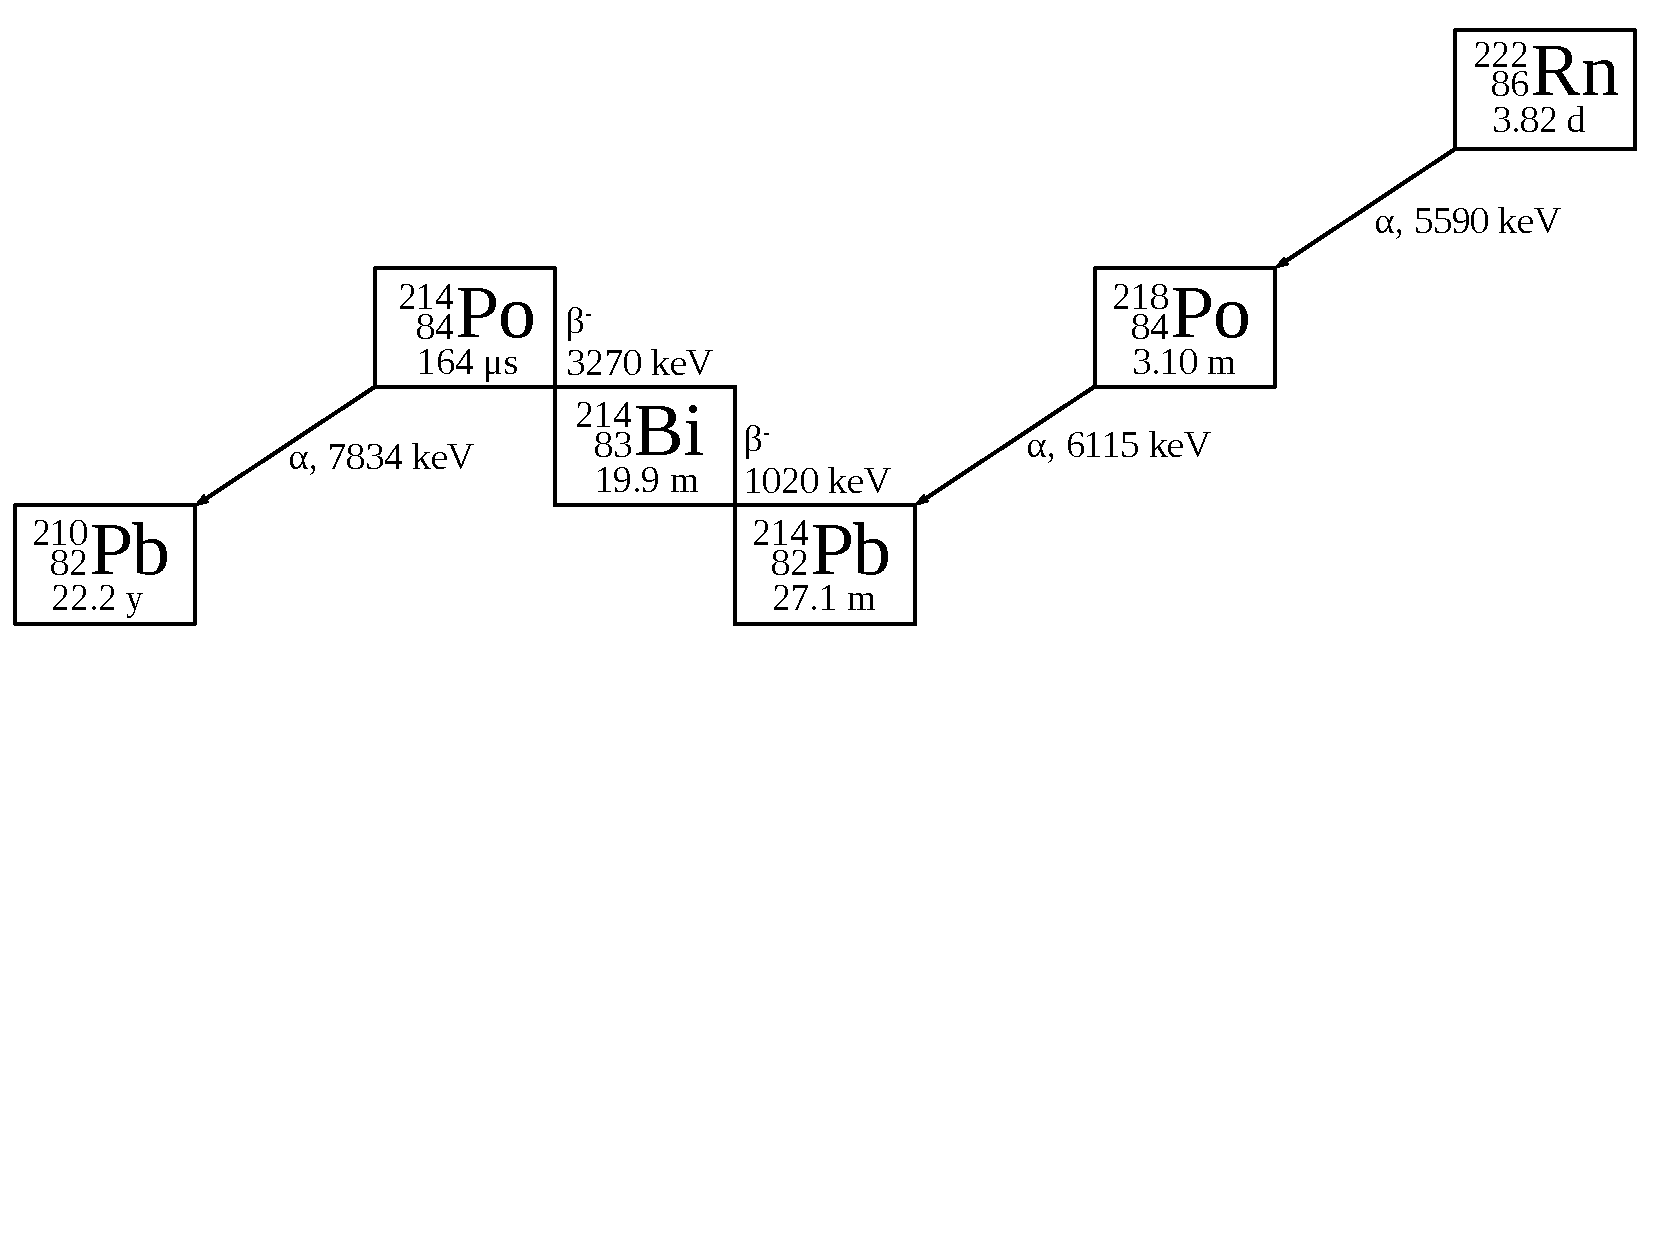
\includegraphics[width=0.8\textwidth, clip=true, trim= 5 295 5 10]{figures/rnveto/decay_scheme_rn222}
    \caption{A section of the decay chain of primordial ${}^{238}$U. Atoms of \Rn~emanate out of impurities in the metals used in detector construction and mix throughout the xenon volume. Low-energy decays of \Pb~that decay directly to the ground state of $^{214}$Bi are the leading source of background in the dark matter ROI~\cite{Aprile:2015uzo}.}\label{fig:useries}
\end{figure}

\subsection{A review of convection}~\label{sec:convec_review}

The two most common types of convection are natural convection, arising from thermodynamically-driven density gradients, and forced convection, arising from the action of a pump or other such device. We will focus here on natural convection, as this dominates over forced convection inside the TPC. Buoyancy-driven convection arises when it becomes more thermodynamically efficient for a fluid volume to transfer energy via mass transfer (moving warmer elements from heat sources to heat sinks) than for heat to move via thermal diffusion. The dimensionless quantities commonly associated with natural convection are the Rayleigh, Grashof, and Prandtl numbers~\cite{Chandrasekhar:1961,Grashof,Prandtl}, given by

\begin{align}
\n{Ra}_x &= \frac{g\beta\Delta T x^3}{\nu\alpha} = \n{Gr}_x\n{Pr} \\
\n{Gr}_x &= \frac{g\beta\Delta T x^3}{\nu^2}\\
\n{Pr} &= \frac{\nu}{\alpha}
\label{eq:dimensionless}
\end{align}

Here, $\n{Ra}$ is the Rayleigh number and $\n{Gr}$ the Grashof number, $g$ the earth's gravitational field ($9.8\1{N/kg}$), $\beta$ the coefficient of thermal expansion ($2.38\times10^{-3}\1{K^{-1}}$), $\nu$ the kinematic viscosity $1.49\times10^{-7}\1{m^2/s}$), $\alpha$ the thermal diffusivity ($6.81\times10^{-8}\1{m^2/s}$), $\Delta T$ the temperature difference ($0.3\1{K}$), and $x$ the chracteristic length scale ($1\1{m}$). $\n{Gr}$ relates buoyancy and viscosity and depends on the details of the volume, while the Prandtl number $\n{Pr}$ is the ratio between viscous and thermal diffusion rates and is a function of the fluid temperature. Unless otherwise noted, values for thermodynamic properties of xenon used in this chapter are from NIST~\cite{NIST}. As a full discussion of the dimensionless quantities used here is beyond the scope of this thesis, the interested reader is recommended to consult any engineering textbook on fluid mechanics and heat transfer. The author found Refs.~\cite{Potter} and~\cite{Holman} particularly useful.

For the Grashof number, the transition between laminar and turbulent flow occurs for $8 < \log_{10}Gr < 9$. For the Prandl number, values less than unity mean thermal diffusivity dominates, and values greater than unity mean momentum diffusivity dominates. If we evaluate the Grashof, Rayleigh, and Prandtl numbers, we find values of $3\times10^{11}$, $7\times10^{11}$, and $2.2$ respectively, which indicate a turbulent flow and momentum diffusivity.

We can compare this to the expectation from forced convection via the Reynolds number~\cite{Stokes}. The two inlet pipes at the bottom of the detector are $10\1{mm}$ in diameter and expand into the $1\1{m}$ diameter of the active region. A recirculation rate of $50\1{slpm}$ corresponds to $300\1{g/min}$ or $5\1{g/s}$ of xenon. With a liquid density of about $3\1{g/cm^3}$, this will correspond to a flow speed of $1\1{cm/s}$ in each pipe. From mass continuity, the velocity decreases by a factor of about 5000 to a bulk average of $10\1{\mu m/s}$. The Reynolds number associated with this velocity is $60$. This corresponds to slow, laminar flow, so the turbulent flow as indicated by the Grashof number will dominate.

\section{Convection in XENON1T}~\label{sec:convection}

Given the similarities in the convection patterns between XENON100 and LUX and the differences between how those experiments inject xenon into the active volume, concrete predictions of what to expect in XENON1T are difficult to make. Conceptually, we might expect a similar single-cell pattern, or the increased detector size might allow the formation of two cells. Thus, it is important that any attempt to measure the convection be as agnostic possible, in order to avoid projecting expectations onto the data.

To measure convection we require two decays out of a decay chain so that there is a meaningful correlation between decay vertices. We further impose a number of requirements on these two decays.
\begin{enumerate}
\item One isotope in the chain must be capable of being injected into the detector and must mix throughout.
\item The two decays of interest must be easily identifiable and shouldn't confuse position reconstruction in any way.
\item The lifetime of the second decay must be relatively short such that $v_{ave}\tau$ is larger than position reconstruction uncertainties, yet small enough such that within two or three lifetimes it's still closer to its parent than any others (to facilitate easy matching).
\item Any further activity in the decay chain must either decay away quickly or be removable (decay is preferable).
\end{enumerate}

Requirememt $(1)$ excludes all decay chains without some gasseous form, or that cannot form some gasseous compound (conceptually similar to $\n{CH}_3\n{T}$ or $\n{UF}_6$). Requirement $(2)$ points towards isotopes that primarily have an $\alpha$-decay mode, as a high-energy $\gamma$ will scatter multiple times, which makes position reconstruction difficult. Isotopes with $\beta$-decays are difficult to identify due to the lack of defining spectral features. Requirement $(3)$ can be fulfilled by reducing the activity of the isotopes in question, but this then means the measurement requires more time. Furthermore, if the lifetime of the second isotope is not short compared to the timescale of convection, this also makes matching difficult, as the effects of curvature of the fluid streamlines will need to be incorporated when the convection map is constructed.

Pairings of radon and polonium are often ideal for this purpose. Both elements tend to decay via $\alpha$ decay and only rarely emit $\gamma$s during the process, which makes clean populations relatively easy to select. Radon, being a noble element, is easy to introduce into the detector and can bypass most purification systems. With the exception of \Rn, radon has no long-lived progeny, fulfilling requirement $(4)$. If this measurement is done at the end of the detector's lifetime requirement (4) can be relaxed, however this would preclude any investigation of changes in the convection pattern over time.

\subsection{$^{220}$Rn-$^{216}$Po}

Given how successful the pairing of $^{220}$Rn and $^{216}$Po were for XENON100 for convection measurements, it is a logical place to start for XENON1T. However, the convection timescale for XENON100 ($\sim2$ minutes) is much shorter than that for XENON1T, so $^{220}$Rn, with only a $55$ second half-life, cannot mix throughout the detector before it decays. Only a paucity of the $^{220}$Rn atoms injected into the active volume reach the drift region, with the majority decaying at or below the cathode.

\subsection{$^{222}$Rn-$^{218}$Po}

Another available option is to match \Po~decays to their parent \Rn~decays. This is a nontrivial endeavour, as the $3.1\1{min}$ half-life of \Po~is quite lengthy. Even at a very modest $1\1{mm/s}$ convection speed, half of all polonium atoms will move tens of centimeters away from their parents. Also, the \Rn~background is both boon and bane. As the radon is mixed uniformly, this provides potential matched pairs in the entire active volume, however several \Rn~events will occur during the lifetime of the average \Po~atom. This increases the probability of forming incorrect matches.

The \Rn~background rate is $14\1{\mu Bq/kg}$, for a total activity in the active volume of $28\1{mBq}$. The population of \Rn~necessary to provide this activity is easily found via $R = \frac{\dd N}{\dd t} = -\lambda N$, where $R$ is the rate, $\lambda = \ln 2/t_{1/2}$ the decay constant, and $N$ the number of atoms. Thus, we find the \Rn~population size is about $13\,300\1{atoms}$. These will mix uniformly throughout the detector, giving an average distance between \Rn~atoms of $3.9\1{cm}$. We apply the same calculations for \Po~and find an average population of $7.5\1{atoms}$. The small number of \Po~atoms means it will be more significantly affected by the normal Poissonian population fluctuations.

\subsubsection{Decay identification}\label{sec:alphaselection}

Selection of \Rn~and \Po~is very straightforward. A plot of the reconstructed $z$-coordinate versus cS1 is shown in Figure~\ref{fig:z_cs1} for the alpha region of interest (ROI).

\begin{figure}[htb]
\centering
    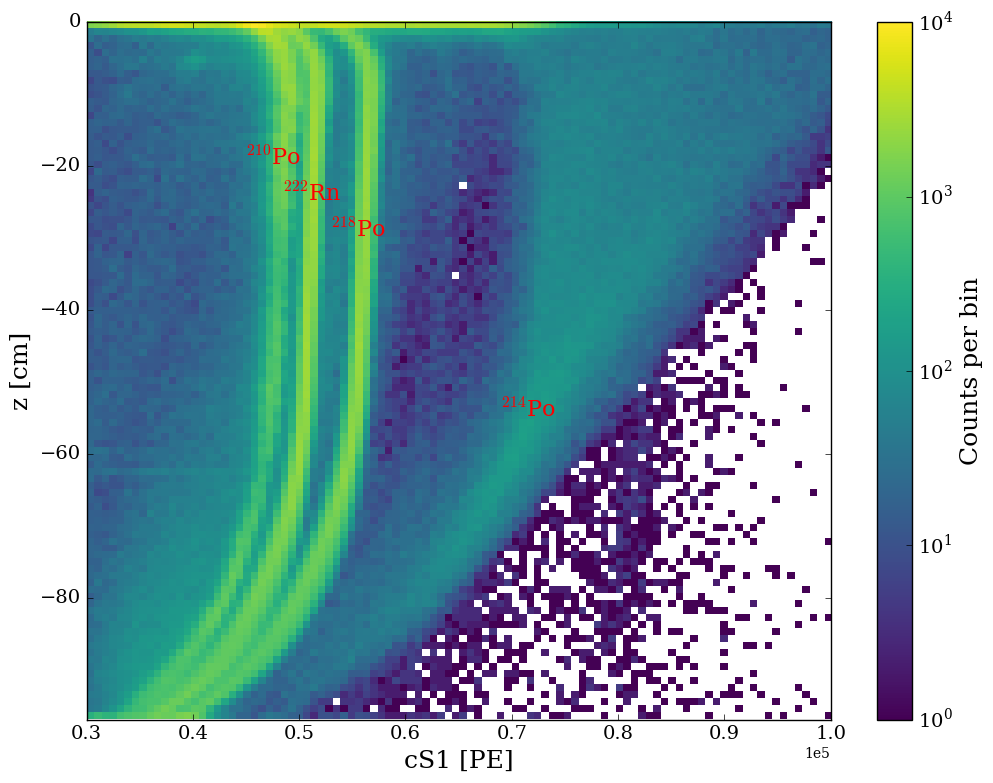
\includegraphics[width=0.8\textwidth]{figures/rnveto/z_cs1}
    \caption{Reconstructed $z$ position versus corrected scintillation light for the alpha ROI. Note the breakdown of the correction factor towards the top and bottom as PMT saturation becomes significant. Four populations are evident in the bulk: $^{210}$Po, \Rn, \Po, and $^{214}$Po. The $^{214}$Po is often misreconstructed due to the topology of \BiPo~events deep in the detector, which smears out its population.}\label{fig:z_cs1}
\end{figure}

The $^{210}$Po population exists nearly entirely on the PTFE reflectors that form the wall of the TPC; a radial cut of even one or two centimeters significantly reduces its size. The $^{214}$Po band shows up much more clearly if one considers \textit{s1\_area\_fraction\_top} rather than $z$, as the short half-life of $^{214}$Po causes some confusion for reconstruction of the $^{214}$Bi-$^{214}$Po (\BiPo) events. The larger S1 from the $^{214}$Po is often paired with the larger S2 from the $^{214}$Bi, resulting in a drift-time that is shorter than the actual value by the lifetime of the $^{214}$Po atom.

As we are primarily interested in the center two populations, we can readily select them in the bulk by drawing a few curves on Figure~\ref{fig:z_cs1}, although this tends to break down close to the cathode or liquid surface as the populations smear together. Alternately, machine learning algorithms can exploit separations in multiple parameter spaces simultaneously, providing some additional selection power in these edge regions (see Appendix~\ref{app:ml}).

After making selections, we find population sizes as given in Table~\ref{tab:alpha_pops}.

\begin{table}[htb]
\centering
    \caption{Number of \Rn~and \Po~alpha decays measured during the first two XENON1T science runs}\label{tab:alpha_pops}
    \begin{tabular}[c]{|l|l|cc|}
        \hline
        Data & Calendar duration & \Rn & \Po \\
        SR0 & 56 days & $78\,519$ & $73\,759$ \\
        SR1 & 369 days & $581\,048$ & $550\,301$ \\
        \hline
    \end{tabular}
\end{table}

\subsubsection{Decay matching}

Armed with reasonably clean populations of \Rn~and \Po, the work of decay matching can begin. To do this with as little bias as possible, we begin by plotting the temporal and spatial separations of all \Rn~and all \Po~pairs in Figure~\ref{fig:dsdt}. As we can see, most of this parameter space is dominated by random, incorrect pairings. Within a minute after a \Rn~decay, its \Po~daughter merges with the bulk population and cannot be identified with an agnostic approach.

\begin{figure}[htb]
\centering
    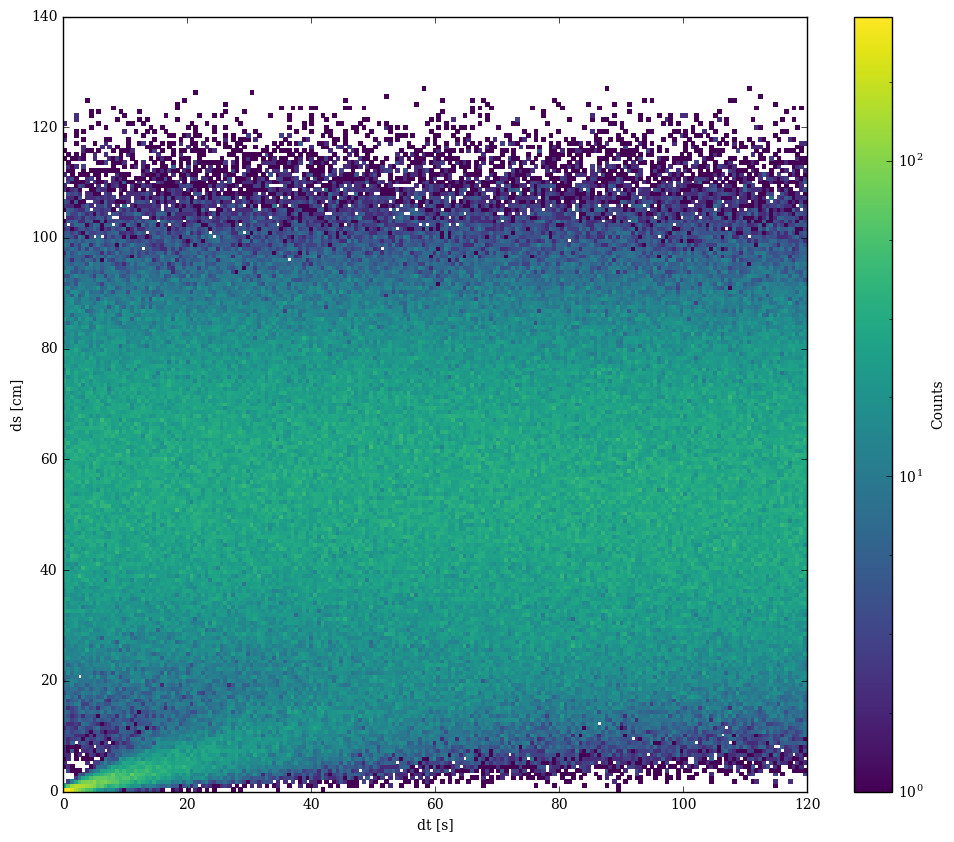
\includegraphics[width=0.8\textwidth]{figures/rnveto/dsdt}
    \caption{Spatial and temporal separations of \Rn~and \Po~events. The ``signal'' population of correct pairs begins at the origin and quickly merges with the ``background'' band of random pairs. Thus, an agnostic approach becomes difficult at times longer than about 45 seconds or distances further than about $15\1{cm}$. Pairs are selected from within the red bounded region.}\label{fig:dsdt}
\end{figure}

To gain the most number of correct matches without being swamped by random matches, we require \Rn~and \Po~matches to be within 30 seconds and 20 centimeters of each other. While this does reduce the amount of background matches, it only allows for $1-e^{-\lambda_{\mathrm{Po}}t} = 10\%$ of all possible correct matches. Additionally, we require matches to be below the line given by $\n{ds} = 3\1{cm} + 0.53\1{cm/s}\cdot\n{dt}$, which is a generous line above the band of correct matches. By setting these requirements, we collect 7855 matches for SR0 and $59\,554$ matches for SR1.

To evaluate the background contamination to this population, we exploit the symmetries in this parameter space. As the background population is flat in time, by repeating the identical matching process but shifting to the left to avoid the signal region, we can quantify the number of background pairs. A shift in time of 35 seconds yields 553 matches for SR0 and 4351 for SR1. This is a background contamination of about $7\%$.

The distribution of speeds is shown in Figure~\ref{fig:speeds}. The median speed is $3.4\1{mm/s}$, and the 10\% and 90\% quantiles are $1.5$ and $6.0\1{mm/s}$, respectively. This is much slower than what was observed in XENON100 and an order of magnitude less than in LUX. The corresponding convection timescale is therefore about 15 minutes.

\begin{figure}[htb]
\centering
    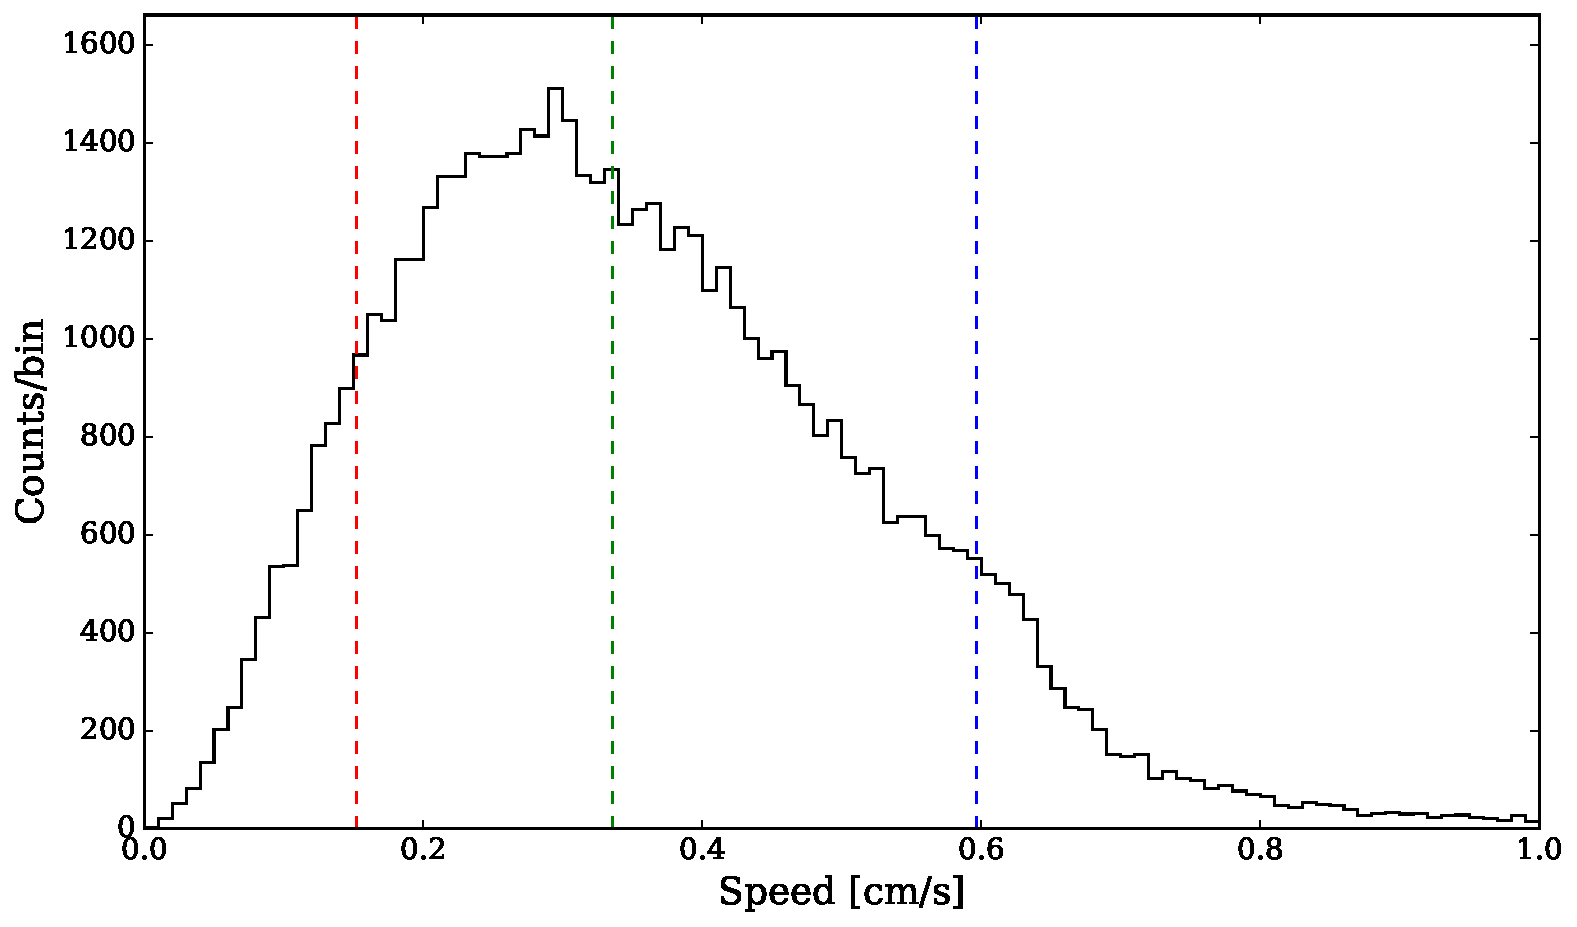
\includegraphics[width=0.8\textwidth]{figures/rnveto/sr1_speed_quantiles}
    \caption{The distribution of \Po~atom speeds in XENON1T. The vertical dotted lines represent the $10\%$, $50\%$, and $90\%$ quantiles.}\label{fig:speeds}
\end{figure}

\subsection{Convection map}

By building a three-dimensional map of the displacement of each matched pair we see the shape of the pattern is, as in XENON100 and LUX, a single cell, with much lower speeds of around $3\1{mm/s}$. Figure~\ref{fig:convec} is a projection approximately along the axis of angular momentum.

\begin{figure}[!p]
\centering
    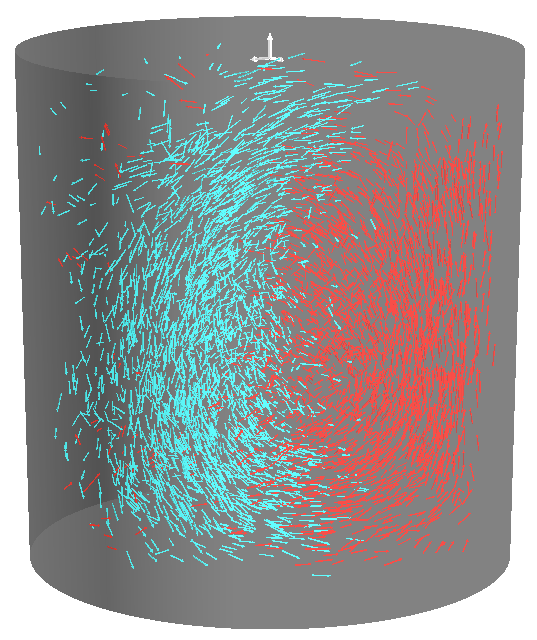
\includegraphics[width=\textwidth]{figures/rnveto/convection_full}
    \caption{The convection field in XENON1T, measured by matching decays of \Rn~and \Po. Red arrows indicates upward movement; blue, downward. A single cell pattern, as was observed in XENON100 and LUX, is clearly seen. Typical speeds are $3\1{mm/s}$. This plot shows approximately one month of data.}\label{fig:convec}
\end{figure}

We also see a lack of matched pairs in the corner regions. It is unlikely that there is no \Rn~there, but it is entirely possible that our event selection requirements perform very poorly here. This also might be interpreted as hints of counter-current eddies forming in the corners of the detector.

Once a preliminary map is made, this can be used to distinguish correct pairings of \Rn~and \Po~from random matches. The vector connecting two decay verticies should be approximately aligned with the convection cell for correct matches and have a random direction for the incorrect matches. Additionally, because there is at most one \Po~for each \Rn, once a given \Rn~or \Po~has been matched, all other potential matches involving either atom can be removed from consideration.

The combination of these effects allows for an interative process where the matches with the smallest separations (having the best signal to background ratio) are chosen, and any other matches involving these are removed, which reduces the background to all further matches. This can be done again with matches with slightly larger separations. However, the efficacy of this iterative technique is limited, because the signal decrease is exponential while the background decrease is merely linear.

\section{Simulation}

The manner of xenon injection in XENON100, LUX, and XENON1T are all different yet all three have the same convection pattern. From this we can conclude that recirculation does not have a significant impact on convection. Thus, a computational fluid dynamics (CFD) simulation can have some predictive power between experiments, as long as the thermodynamic boundary conditions are correctly modeled. Additionally, a convection field from simulation may reveal more about the underlying detector operation than measurements from data.

A variety of different software packages, commercial and otherwise, are available to do this kind of simulation. ANSYS Fluent~\cite{fluent} was used for this work on advice from professor Carlo Scalo of Purdue engineering, and it is available on the Purdue computing clusters.

A simplified full-size model of the active volume was used to build the simulation mesh with $10^6$ nodes, and thermodynamic data from NIST~\cite{NIST} was used for the properties of liquid xenon at the operating conditions of the detector. The Boussinesq approximation~\cite{Boussinesq:1897} was used to model the density, which ignores changes in density except in terms also containing $g$, the Earth's gravitation field. As we expect slow, buoyancy-driven flows, the approximation is valid. Temperature values were based on slow control measurements from XENON1T in the period of 18-21 June, 2017, though it should be noted that only one of the temperature sensors is mounted inside the active region, with the remainder outside the PTFE reflectors. The values used were $176.9\1{K}$ at the bottom of the detector and $177.1\1{K}$ at the top. Heat input from the bottom PMT array was taken as $0.25\1{W}$. A steady-state solution was simulated, using a pressure-based solver and absolute velocity formation. The solution methods used were the third-order MUSCL method for energy and momentum, and pressure-driven density changes calculated via the Navier-Stokes equations. A representative result is shown in Figure~\ref{fig:cfd_sample}.

\begin{figure}[htb]
\centering
    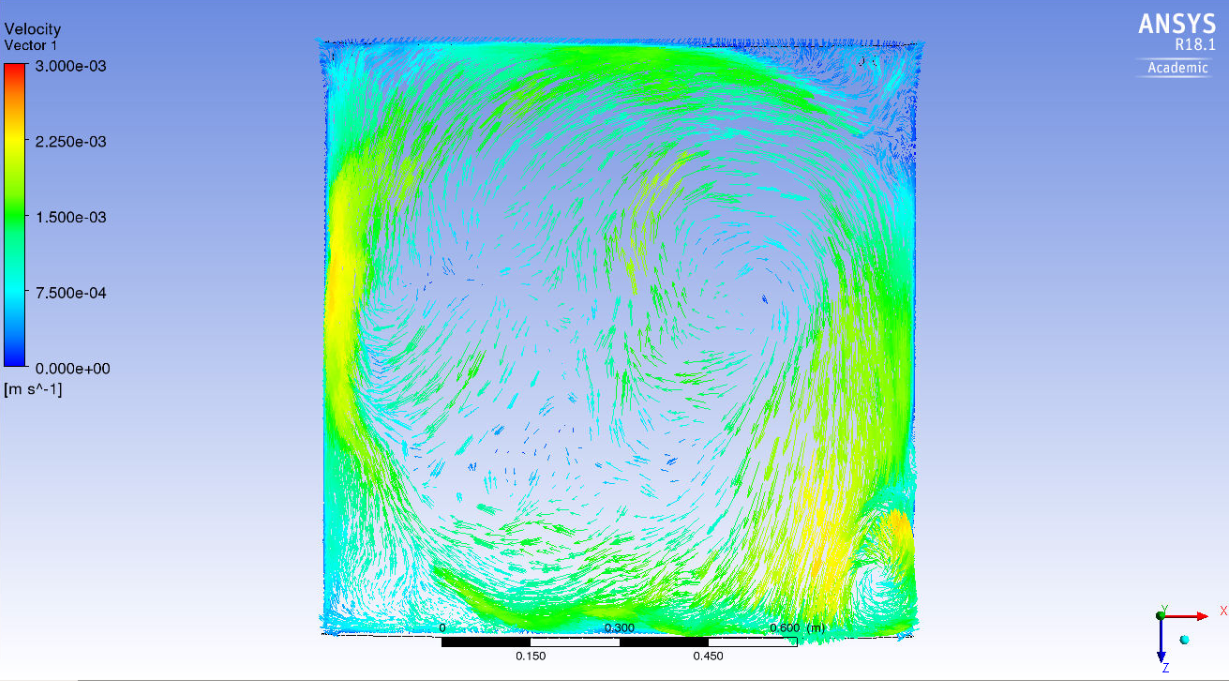
\includegraphics[width=0.8\textwidth]{figures/rnveto/convection_sim}
    \caption{Simulated convection pattern for XENON1T. A single large cell is evident with speeds of a few mm/s. A simple temperature gradient is sufficient to drive this system, though the mechanisms that determine the direction of angular momentum is not yet understood. Counter-currents can be seen in the corners.}\label{fig:cfd_sample}
\end{figure}

A transient simulation was also performed to investigate possible short-term deviations from the steady-state behavior. While the results agree qualitatively with each other, vortex shedding from counter-currents in the corners were routinely observed in the transient solution.

\section{Comparison between simulation and data}

The simulation results agree qualitatively with the data. A simple temperature gradient is sufficient to establish and drive a single-cell convection pattern, although the symmetry-breaking mechanism that determines the orientation of the pattern is not yet understood. No correlation has been found between the layout of pipes to and from cryogenics and purification and the direction of cell angular momentum. Additionally, the spatial distribution of speed between data and simulation are in disagreement. In the simulations, the highest speeds are very close to the walls, and the center region is fairly quiet, while in data the speeds are much more homogonously distributed.

\section{The radon veto}~\label{sec:rnveto}

If it is possible to follow atoms of \Po~around the detector, the next step is to follow atoms further down the decay chain. If \Pb~atoms can be followed and their decays identified, these events can be removed from the analysis. As \Pb~is the dominant background source in the dark matter region of interest~\cite{Aprile:2015uzo}, removing these events lowers the overall background rate, which will improve the sensitivity of the experiment at a marginal exposure cost. We exploit the fact that because \Pb~is part of a decay chain, the times and positions of its decays have physical significance to the atoms surrounding it.

\subsection{Technique overview}

While there is nothing about a \Pb~event that is easily identifiable, its parent isotopes (\Rn, \Po) and daughter (\BiPo) can be identified with relative ease using alpha spectroscopy or the BiPo timing structure~\cite{Aprile:2017fhu}. This allows us to bookend the \Pb~event with events that are more easily identified. With this information, an algorithm resembling one for track reconstruction can be employed to improve the confidence with which \Pb~events are tagged by identifying the decays of the parents and daughter and looking for the convection streamlines that connect them. The \Pb~decay must happen somewhere on the streamline between the \Po~and \BiPo~decays. A stylized representation of this is shown in Figure~\ref{fig:rnveto_schematic} where displacement due to convection is normalized out.

\begin{figure}[htb]
\centering
    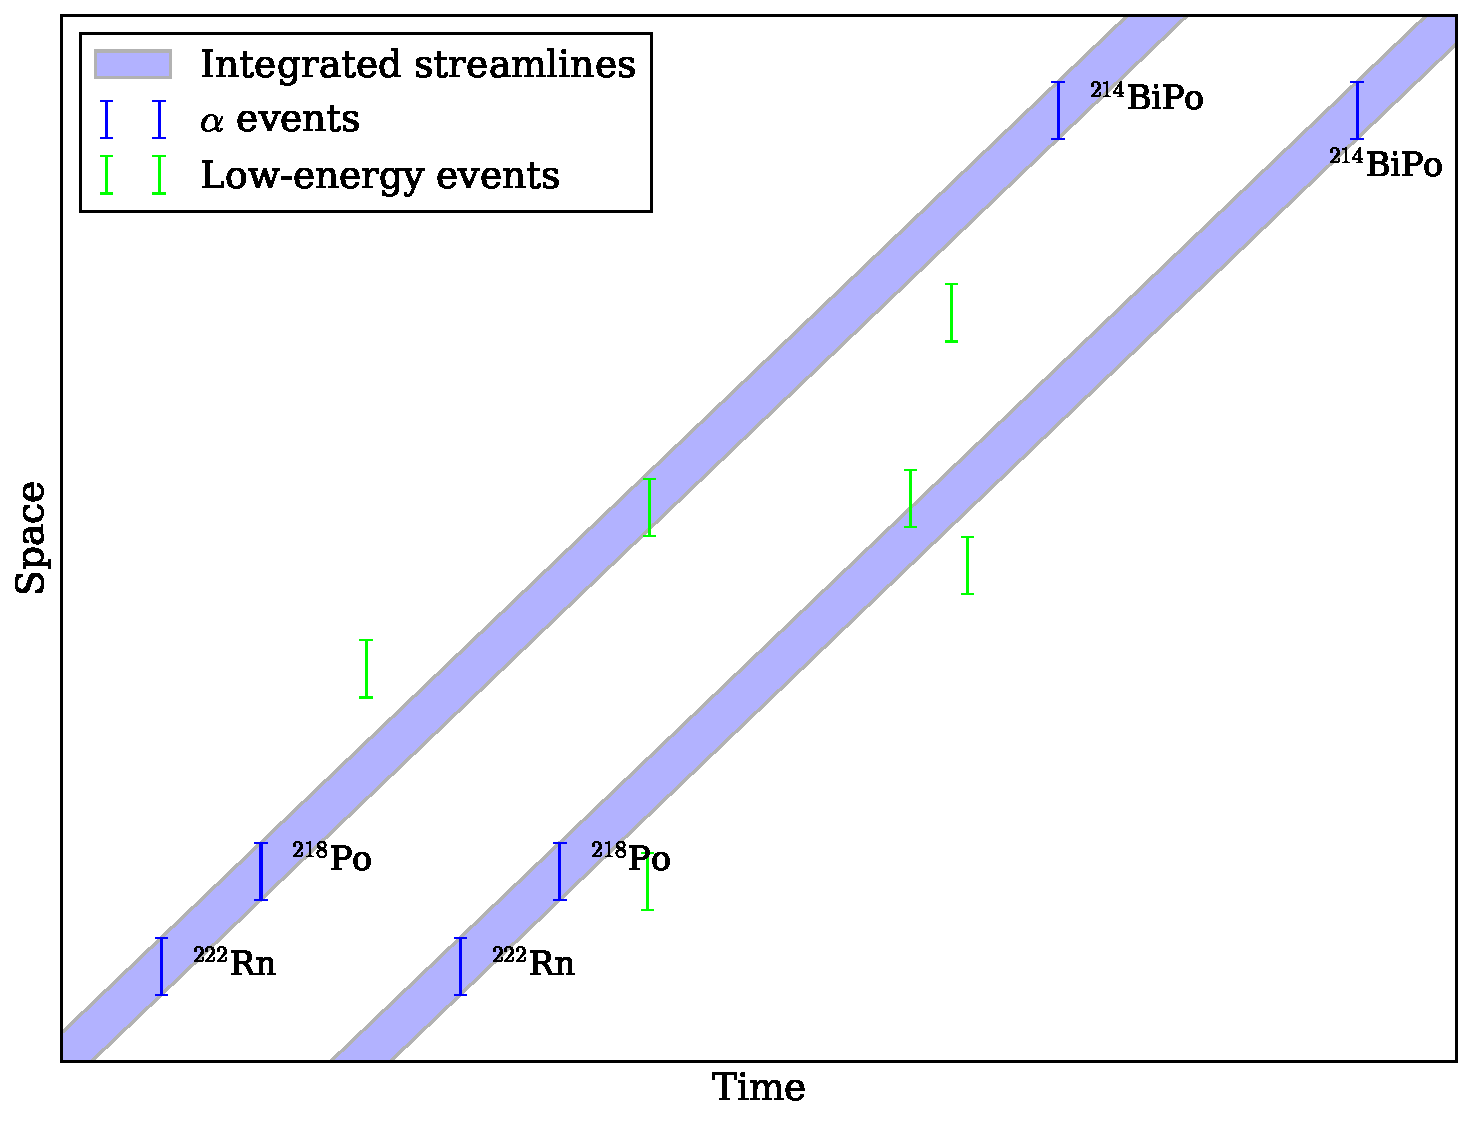
\includegraphics[width=0.8\textwidth]{figures/rnveto/rnveto_schematic}
    \caption{A simple schematic of how the radon veto works. Low-energy events (in red) due to \Pb~can be identified because they occur on streamlines (shaded regions) connecting \Rn, \Po, and \BiPo~events (in blue), while low-energy events due to other background sources occur at random.}\label{fig:rnveto_schematic}
\end{figure}

\subsection{Convection-agnostic approach}

To demonstrate a proof of this concept, we apply a convection-agnostic approach to XENON1T SR0. In this method, a growing sphere is placed around the vertex of every \Po~or \BiPo~event and the sphere is watched to see if a low-energy event occurs within it. As the knowledge of convection is not yet sufficient to accurately integrate the position of the \Po~or \BiPo, the center of the sphere remains in a fixed location. Regardless of the size of the sphere or how long one watches it, some fraction of \Pb~decays will occur within it. The rate of growth of the sphere can be set from convection (we take $0.6\1{cm/s}$, the 90th percentile of convection speed), and the observation time can be chosen by a simple optimization to maximize the potential background reduction while minimizing the overall exposure cost. The background reduction is proportional to $1-e^{-\lambda t}$, using the decay constant of \Pb~for the \Po-veto, and $^{214}$Bi for the \BiPo-veto. The exposure cost from these spheres is proportional to $t^4$.

\Po~events are selected as in Section~\ref{sec:alphaselection}, \BiPo~events following the method in~\cite{Aprile:2017fhu}, and low-energy events following the developed XENON1T analysis selection criteria~\cite{Aprile:2017iyp} (for a detailed description of one of them, see Appendix~\ref{app:s1aft}), with the difference that events are selected up to $150\1{keV}$. Events in the energy region near the $41\1{keV}$ line from $^{83m}$Kr were cut to remove contamination from this calibration isotope, and the region between 50 and $80\1{keV}$ is blinded for the $^{124}$Xe double electron-capture analsis. All events are required to lie within the 1.3~tonne fiducial volume. We find event populations of $48\,721$ for \Po, $16\,485$ for \BiPo, and 974 in the low-energy region.

\begin{figure}[htb]
    \centering
    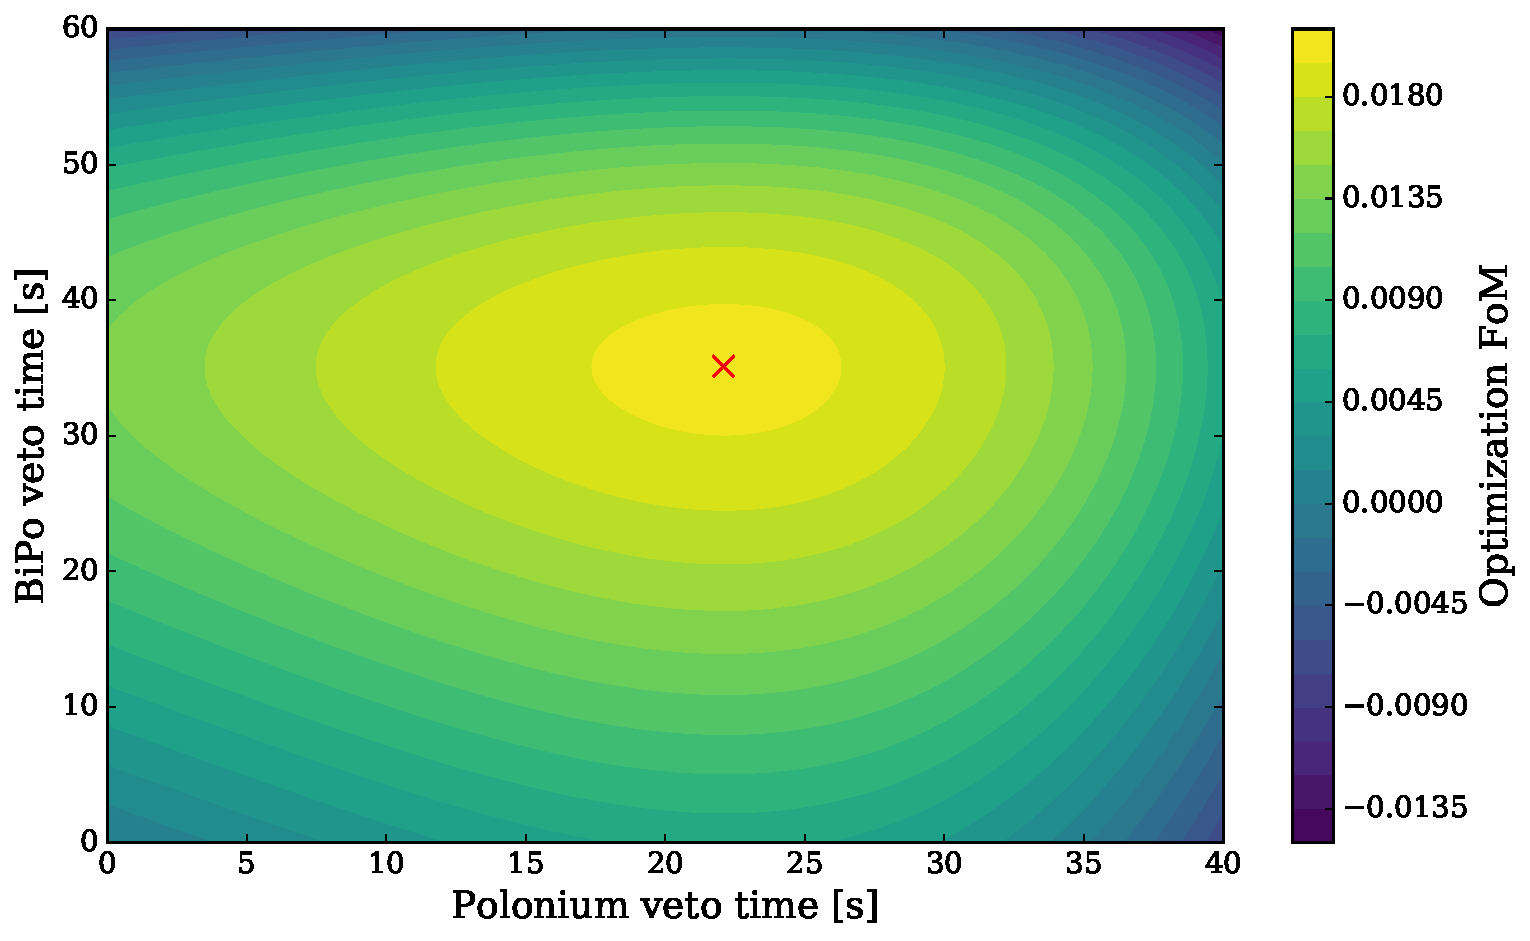
\includegraphics[width=0.8\textwidth]{figures/rnveto/sr0_veto_time_optimization}
    \caption{A simple optimization to find the best veto times for \Po~and \BiPo~events from SR0. The figure of merit used here is the difference between the total background found (proportional to $1-e^{-\lambda t}$) and the fractional exposure cost (proportional to $t^4$). The best value is marked with the red `x', corresponding to times of $22.1\1{s}$ for \Po~and $35.1\1{s}$ for \BiPo. These are background reductions of $0.8\%$ for \Po~and $1.8\%$ for \BiPo~(total $2.7\%$). The exposure cost is $0.66\%$.}\label{fig:veto_time_optimization}
\end{figure}

The optimal veto times for SR0 are $22.1\1{s}$ and $35.1\1{s}$ for \Po~and \BiPo, respectively. These correspond to background reductions of $0.8\%$ and $1.8\%$, respectively, and a combined exposure cost of $0.66\%$ ($279\1{kg\cdot day}$).

\Pb~events are selected by placing these growing spheres around \Po~and \BiPo~events. Any low-energy event that happens within the boundary in space and time defined by this sphere is tagged.

The principle background to this Big Sphere method is that of false positives from random coincidence. This can be quantified through a simple Monte Carlo by doing this analysis at random locations and random times within the detector, and counting the number of observed events. Alternately, locations and timestamps of \Po~and \BiPo~events can be used, but the search can be done by looking before \Po~and after \BiPo~(ie, where the \Pb~cannot be). The Monte Carlo method allows for the creation of a background distribution, which means we can easily quantify the significance of the result when we look for \Pb~events from \Po~and \BiPo~events. We perform this analysis at random locations and times a total of $10^{5}$ times for each isotope. The background distributions are very well described by Poisson distributions, with shape factors $\mu_{Po} = (1.232 \pm 0.004)$ and $\mu_{BiPo} = (2.411 \pm 0.005)$, as shown in Figure~\ref{fig:bs_sr0}.

\begin{figure}[htb]
\centering
    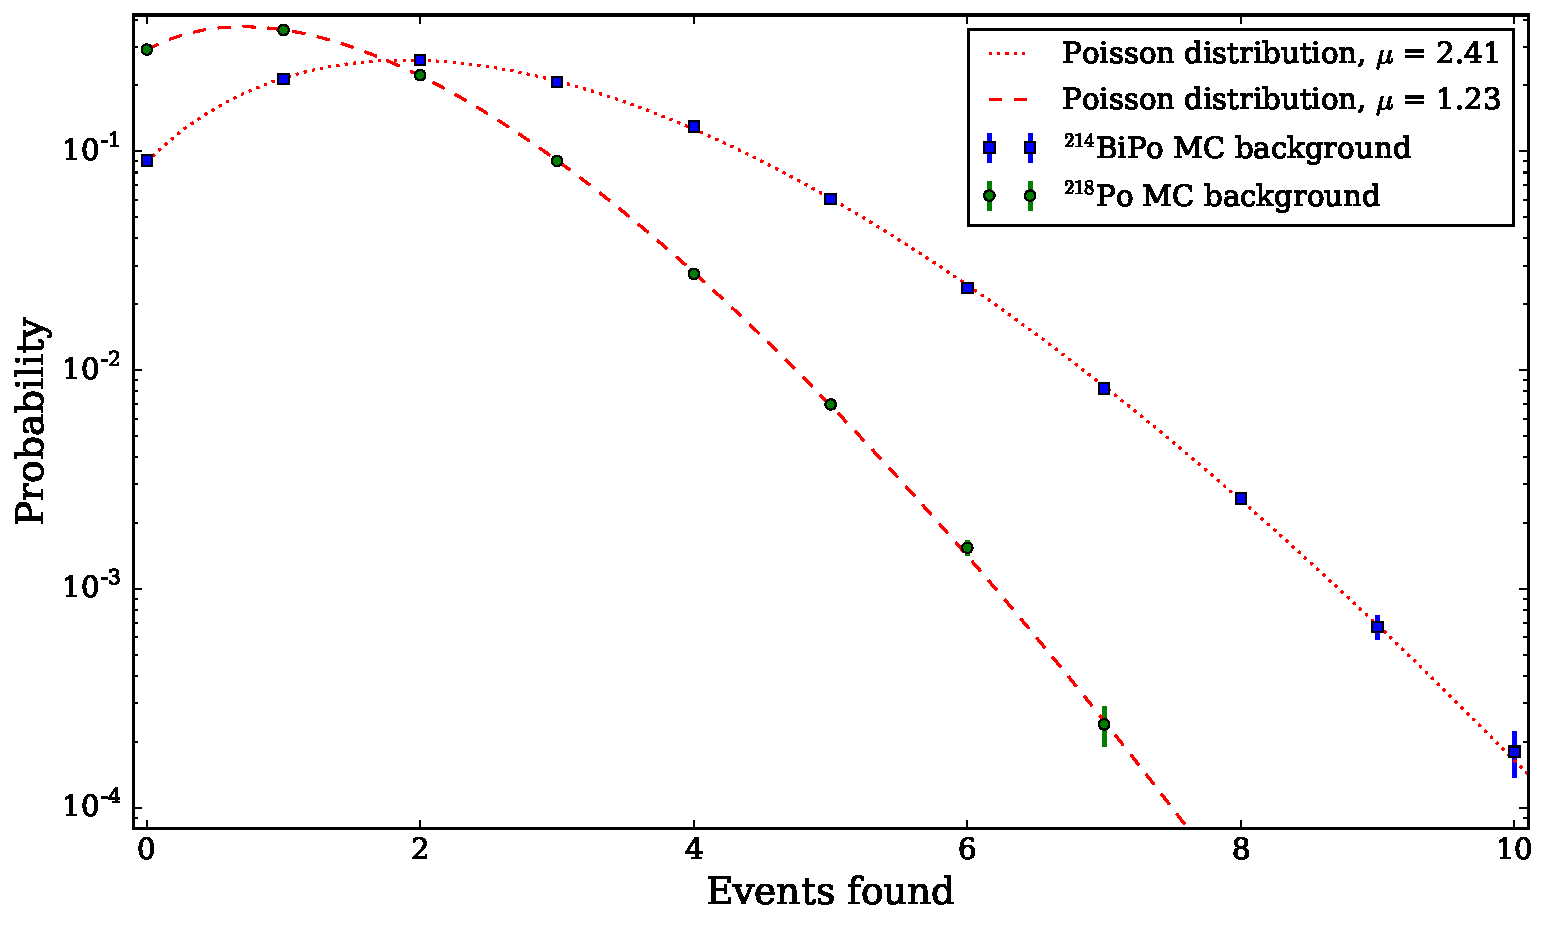
\includegraphics[width=0.8\textwidth]{figures/rnveto/sr0_bigsphere_bkg}
    \caption{The simulated background expectation for the convection-agnostic Big Sphere radon veto method applied to SR0. The background from false positives is well-modeled with a Poisson distribution with shape factors $\mu_{Po} = (1.232 \pm 0.004)$ and $\mu_{BiPo} = (2.411 \pm 0.005)$. The number of events found by searching near \Po~is 8 and \BiPo~is 5. These have p-values of $6.0\times10^{-6}$ and $3.6\times10^{-2}$, respectively, indicating that the Big Sphere method is statistically better than selecting events at random.}\label{fig:bs_sr0}
\end{figure}

If we apply this technique to the physically motivated locations and times of \Po~and \BiPo~events, we find 8 events from \Po~and 5 events from \BiPo. Looking in the opposite directions in time (before \Po~and after \BiPo) we find 3 and 2 background matches, respectively. Using the background distributions as determined by Monte Carlo, these are significant with p-values of $6.0\times10^{-6}$ and $3.6\times10^{-2}$, respectively.

We must now inspect these events to acertain the quality of these matches. If events cluster in suspicious ways we must then be skeptical of the results, but if they are more or less uniformly distributed we can have more confidence in the results. The most important parameter spaces to investigate are those of space, time, and energy, and we show the distributions of the main population of events in Figures~\ref{fig:match_parameters0} and~\ref{fig:match_parameters1}, along with both the correctly and incorrectly vetoed events. We see there are no suspicious groupings of events.

\begin{figure}[htbp]
\centering
    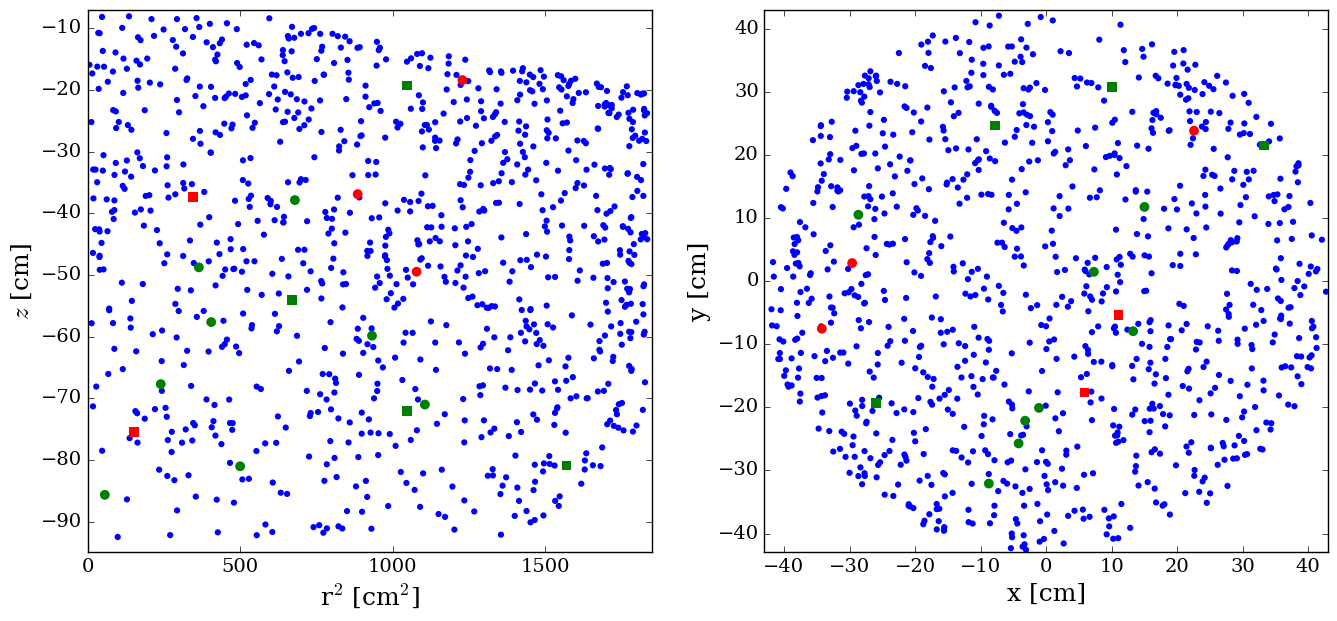
\includegraphics[width=\textwidth]{figures/rnveto/sr0_bs_results_space}
    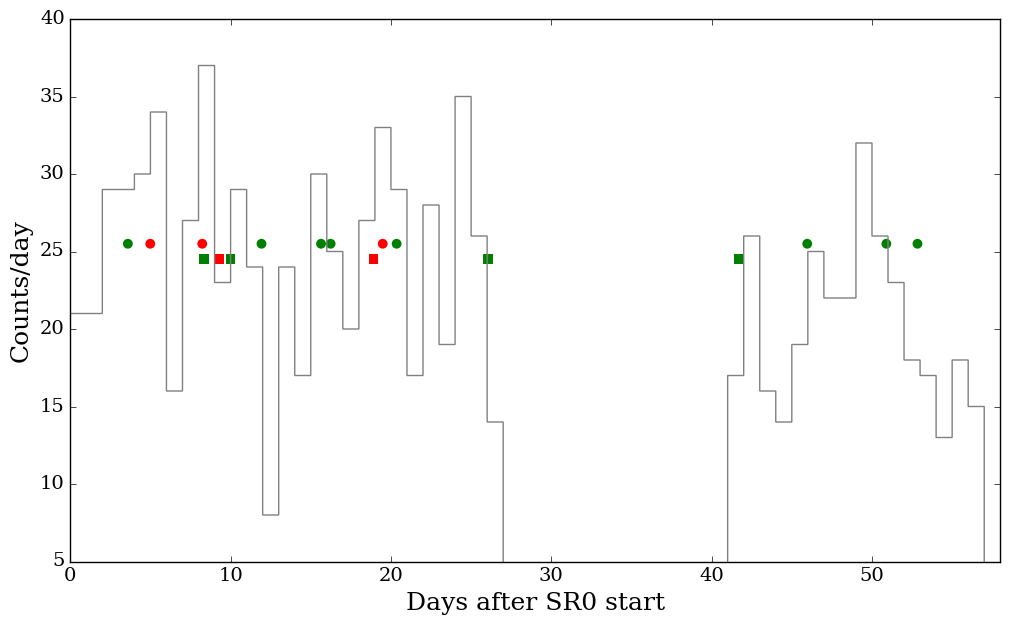
\includegraphics[width=\textwidth]{figures/rnveto/sr0_bs_results_time}
    \caption{Results for the Big Sphere radon veto technique for SR0. The low-energy event population is shown in blue, green circles are events matched after \Po~(correctly matched), red circles matched before \Po~(incorrectly matched), green x's are events matched before \BiPo~(correctly matched), and red x's are matched after \BiPo~(incorrectly matched). Events are distributed uniformly in both space (top) and time (bottom).}\label{fig:match_parameters0}
\end{figure}

\begin{figure}[htbp]
\centering
    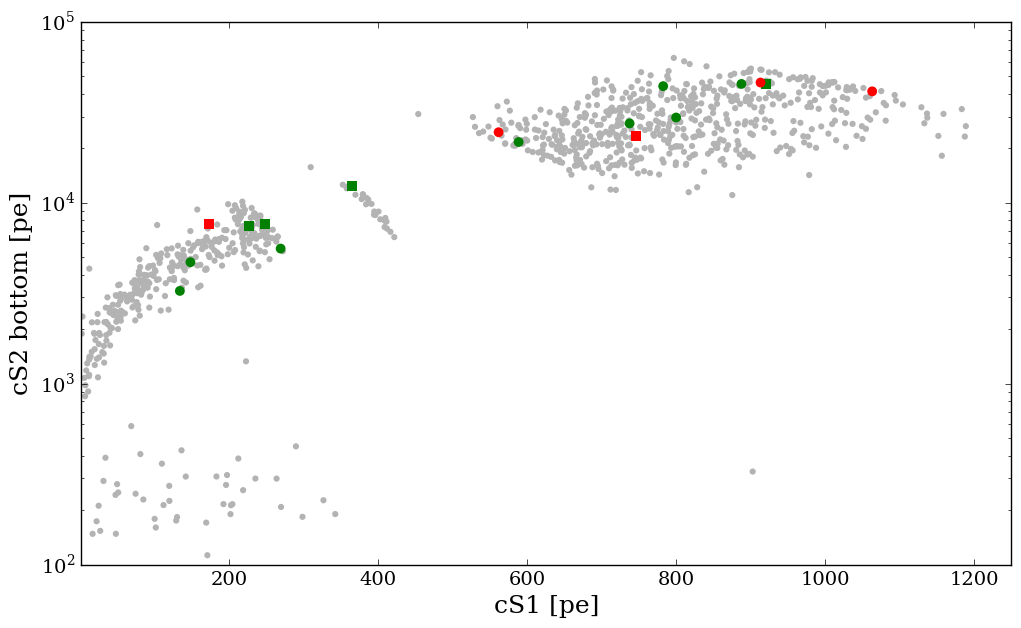
\includegraphics[width=\textwidth]{figures/rnveto/sr0_bs_results_energy}
    \caption{Results for the Big Sphere radon veto technique for SR0. The low-energy event population is shown in blue, green circles are events matched after \Po~(correctly matched), red circles matched before \Po~(incorrectly matched), green x's are events matched before \BiPo~(correctly matched), and red x's are matched after \BiPo~(incorrectly matched). The events are uniformly distributed in energy/discrimination, although none of the matched events lie in the energy ranged used in the dark matter search ($<70\1{pe}$ in cS1).}\label{fig:match_parameters1}
\end{figure}

With the highly significant result from the \Po~matching, this means that this technique is significantly better than merely selecting events at random, and this is sufficient to demonstrate that this technique works. What remains now is to scale up beyond this first convection-agnostic approach.

\subsection{Cloud approach}

The Big Sphere method has a number of limitations. Looking in all directions rather than just along the convection streamlines wastes a large amount of exposure, and in cases where multiple low-energy events are observed within the sphere it is impossible to proceed. At most one can be due to \Pb, yet without additional information it is impossible to determine which. This additional information can be found from convection. If an event is on fluid streamlines originating from the \Po~decay vertex or converging to the \BiPo~vertex, it is more likely to be \Pb~than if it occurred far from those streamlines or on otherwise impossible paths.

Following these streamlines requires numerically integrating the convection vector field. The computational cost of this is non-trivial. Each \Rn~atom can potentially produce a low-energy \Pb~event, so streamlines around every \Rn~must be followed. A tonne-year of exposure will contain about $500\,000$ total \Rn~events, and streamlines from each of these events must be integrated for (on average) one hour, at sufficiently small timesteps to minimize integration errors. By far the most expensive portion of this is the vector field interpolation, which can take a few milliseconds every time. Additionally, one must have a high-resolution and high-accuracy map of the convection field. Without this, errors from interpolation and extrapolation can quickly accumulate and the integrated volume can easily cover large portions of the detector.

\subsection{Diffusion-limited case}\label{sec:difflimit}

The dominant uncertainties at this point to the radon veto stem from the lack of sufficiently detailed knowledge of the convection pattern. However, we can explore the possibilities of the technique should a perfect understanding of convection be obtained. In this limit, the dominant uncertainties are from position reconstruction and diffusion.

\subsubsection{Diffusion effects}

When an event happens inside the detector, we reconstruct its interaction vertex with a uncertainty of $5\1{mm}$ in r and $1\1{mm}$ in z. For reasons we will discuss shortly, we will take 2 sigma and double these values. Thus, we assume this event happens somewhere in a cylinder of volume $\approx 630\1{mm^3}$. This cell will follow the convection lines through the volume, growing in time due to diffusion. We'll need a few values here:
\begin{itemize}
\item $r_0 = 10\1{mm}$
\item $h_0 = 2\1{mm}$
\item Cell volume: $V(t=0) = \pi r_0^2h_0 = 630\1{mm^3}$
\item Diffusion constant: $D = \frac{k_BT}{6\pi\eta r} = 1.7\times10^{-3}\1{mm^2/s}$
\end{itemize}

We find the diffusion constant via the Stokes-Einstein relation for a spherical particle diffusing through a fluid at low Reynolds number~\cite{Sutherland:1905,Einstein:1905,Smoluchowski:1906}. $\eta$ is the viscosity ($0.5\1{mPa\,s}$~\cite{Legros:1965}) and $r$ is the radius of the particle in question (taken as $0.15\1{nm}$). The displacement of the atom from its initial location will be roughly given by $\Delta s = \sqrt{\pi Dt}$, and the increase in volume can be found by adding $\sqrt{\pi Dt}$ to both r and z. Thus

\begin{equation}
V(t) = \pi(r_0 + \sqrt{\pi Dt})^2(h_0 + \sqrt{\pi Dt})
\end{equation}

Starting from a decay of \Po, in one half-life of its daughter ($\sim$30 min) the cell volume will increase by $2.1\1{cm^3}$ to a total of $2.75\1{cm^3}$. If we see an ER event in this volume in the energy range we would expect from a \Pb~decay, we can cut this event (and stop following that cell as the lead atom inside it is now bismuth).

\subsubsection{Total vetoed volume}

The next value to calculate is what fraction of the active region we can follow. For that we need to calculate how many atoms we need to follow at any one time. As calculated above, we find that on average the detector will contain these populations:
\begin{itemize}
    \item $N_{Rn} = 13\,300$
    \item $N_{Po} = 7.5$
    \item $N_{Pb} = 66$
    \item $N_{Bi} = 48$
\end{itemize}

Atoms further down the decay chain will have slightly reduced populations due to plateout and cathode cleaning, but these values are upper limits. The probability that we must still follow the atom in that volume is $P(t) = e^{-\lambda t}$ (if the atom decays, we no longer need to follow it), and the expression for the cell volume is given above.

If we wish to reduce the contribution of \Pb~to the low-energy background to the level where it becomes equivalent or subdominant to the other sources of ER background, we need to veto about 90\% of all low-energy lead events. This means we have to follow a cell for 3 or 4 half-lives, and for this reason we took 2 sigma of the position uncertainty (giving us 95\% of the atoms). The results change very little if we follow the atom around for an infinite number of half-lives, so we will integrate over all time, not just the few half-lives we need, which results in convenient closed-form expressions.

To find the average cell volume we integrate the volume $V(t)$ with the probability density $P(t) = \lambda e^{-\lambda t}$ to get

\begin{equation}
\left< V \right> = \int_0^{\infty} \dd t\,V(t) P(t) = \int_0^{\infty} \dd t\,\pi(r_0 + \sqrt{\pi Dt})^2(h_0 + \sqrt{\pi Dt})\lambda e^{-\lambda t}
\end{equation}

The result is

\begin{equation}
\left< V \right> = V_0 + a\sqrt{\chi} + b\chi + c\chi^{3/2}
\end{equation}

where
\begin{itemize}
    \item $\chi = \frac{D}{\lambda}$ (units of $\n{mm^2}$)
    \item $a = \frac{\pi^{2}}{2} (r_0^2+2 r_0 h_0) = 690\1{mm^2}$
    \item $b = \pi^2 (2r_0 + h_0) = 220\1{mm}$
    \item $c = \frac{3}{4} \pi^{3}$
\end{itemize}

For \Pb, $\chi = 4\1{mm^2}$, so $\Delta V = 2.5\1{cm^3}$ or the total volume we must follow per atom is $V_0 + \Delta V = 3.1\1{cm^3}$. Given the average number of \Pb~atoms we expect to have, this will be a total vetoed volume of $200\1{cm^3}$. This is only $10^{-4}$ of the total active volume, and vetoing these volumes has a negligible cost in exposure. We can also calculate the total volumes to track for the parent and daughter isotopes, but this is only for tagging purposes as we have no need to veto events that aren't \Pb.

If we take a pessimistic approach where we follow each cell for four half-lives (regardless of whether or not the atom in it decays), we find a total vetoed volume of $V(4T_{1/2}) = 300\1{cm^3}$. Thus, the $200\1{cm^3}$ value is reasonable from this point as well.

\subsubsection{Effect of the drift field}

We expect the drift field to cause the motion of any charged daughtber products to diverge from that of the xenon bulk. This effect can be simulated, but measuring the charge on the daughter ion will be difficult, and this uncertainty reduces the effectiveness of any simulation involving this aspect. In effect, it will cause a net downward motion, which will move the ion into other streamlines (or potentially plate onto the cathode). Additionally, as we inject the liquid below the cathode, ions in the liquid may have difficulty passing through the cathode mesh and into the drift region.

EXO-200 found~\cite{Albert:2015vma} radon daughter ion drift speeds of $\sim 1\1{mm/s}$ at a drift field of $350\1{V/cm}$, with ion neutralization time proportional to the electron lifetime. Additionally, they measured the fraction of radon chain decays that leave the daughter in an ionized state. In XENON100 the ion drift was a small correction to the $\sim 8\1{mm/s}$ speed of convection. The relatively low drift field ($\order{100}\1{V/cm}$) in XENON1T means ion drift will be even less signficant.

\paragraph{Conclusion}

The radon veto provides a method to reduce the radon background of XENON1T via an offline analysis. A convection-agnostic proof of concept was presented and demonstrates the potential of this technique. The fundamental diffusion-limited implementation was discussed, but the convection pattern is not yet sufficiently understood to allow for the tracking of ions beyond a few minutes. This remains a topic of interest, and will be the focus for future studies.
